% !TEX program = xelatex
\documentclass{ctexart}%文档类型
\usepackage{amsmath, amsthm, amssymb, graphicx, geometry}%数学公式,图形
\usepackage[bookmarks=true, colorlinks, citecolor=blue, linkcolor=black]{hyperref}%超链接
\usepackage[european]{circuitikz}%电路图
\usepackage{steinmetz}%用于表示幅角
\usepackage{multirow}%用于表格合并单元格
\usepackage{tikz}%用于画图
\usepackage{wrapfig}%用于插入并排两张小图片
\usepackage{geometry}%用于设置页边距
%\usepackage{indentfirst}%用于首行缩进

%\setlength{\parindent}{0em}%首行缩进
\date{}
\linespread{1.5}%行间距
\title{电工学期末复习总结}
\author{Flower}
\geometry{
    a4paper,
    total={170mm,257mm},
    left=20mm,
    }%设置页边距



\newtheorem{theorem}{定理}[section]
\newtheorem{definition}[theorem]{定义}
\newtheorem{lemma}[theorem]{引理}
\newtheorem{corollary}[theorem]{推论}
\newtheorem{example}[theorem]{例}
\newtheorem{proposition}[theorem]{命题}



\begin{document}
\maketitle
\begin{center}
    期末考试临近,希望能够通过这样的
形式快速高效的学会电工学的内容。之
前使用Markdown写了一些笔记,但发现
Markdown对打印不太友好,于是就想着用
\LaTeX{}来写这个总结。
\end{center}
\begin{flushright}
    \begin{tabular}{c}
        Flower\\
        2023年6月
    \end{tabular}
\end{flushright}

\newpage
\tableofcontents
\newpage

\section{直流电路}

\subsection{基本概念}

\subsubsection{作用和组成}

电路的作用:能量的输送与转换(强电),信号的处理与传输(弱电)。

电路的基本组成:电源、负载、连接导线。

概念:电源、负载、导线、内电路、外电路、直流电路(DC)、交流电路(AC)、

\subsubsection{基本物理量}

\begin{center}
    \fbox{不随时间变化的物理量用大写字母,随时间变化的物理量用小写字母}
\end{center}

\begin{center}
    \begin{circuitikz}
        \draw (0,3) node[left]{$+$} 
            to[battery1, l=$U_s$, a=$E\uparrow$] (0,0)node[left]{$-$}
            to[short] (3,0) node[right]{$-$}
            to[lamp] (3,3) node[right]{$+$}
            to[short] (1.5,3) node[above]{$\overset{I}{\longrightarrow} $}
            to[short] (0,3);
    \end{circuitikz}
\end{center}

\begin{enumerate}
\item 电流,电流方向是正电荷的流动方向。
\[
    I = \frac{Q}{t}
\]
\[
    i = \frac{\mathrm{d} q}{\mathrm{d} t} 
\]

\item 电位 

电场力将单位正电荷从电路某一点移至参考点所消耗的电能,也就是在移动中转化非电形态
能量的电能称为该点的电位。

\item 电压

电场力将单位正电荷从电路某一点移至另一点所消耗的电能,即转化为非电形态
能量的电能称为这两点的电压。

方向:从高电位指向低电位。

\item 电动势

电源中的局外力(即非电场力)将单位正电荷从电源负极移至电源正极所换来的电能称为电
源的电动势。

方向:从电源负极指向电源正极,即低电位指向高电位。

\item 电功率

电路中单位时间所转化的电能消称为电功率,简称功率。

电源产生的功率
\[
    P_E=EI
\]
电源输出的功率
\[
    P_s=U_sI
\]
负载功率
\[
    P_L=U_LI
\]

\item 电能

在时间$t$内转化的电功率称为电能。

\[
    W=Pt
\]

\end{enumerate}

\subsubsection{电路状态}

电路状态主要有三种:通路‘开路和短路。

\subsubsection{参考方向}

\begin{center}
    \fbox{电压与电流选取的参考方向应保持一致}
\end{center}

\subsubsection{理想电路元件}

\begin{enumerate}
    \item 理性有源元件
    \begin{itemize}
        \item 电压源 电压恒定
        \item 电流源 电流恒定
    \end{itemize}
    \item 理想无源元件
    \begin{itemize}
        \item 电容
        \[
          C=\frac{q}{u}  \]
          瞬时功率
          \[
            P=ui=Cu\frac{\mathrm{d}u}{\mathrm{d}t}\]
          存储电场能
          \[
            W_e=\frac{1}{2}CU^2\]  
        \item 电感
        \[
            L=\frac{\Psi}{i}\]
          瞬时功率
          \[
            p=ui=Li\frac{\mathrm{d}i}{\mathrm{d}t}\]
            存储磁场能
            \[
                W_m=\frac{1}{2}LI^2
                \]
        \item 电阻
        \[
            R=\frac{u}{i}
            \]
        \[
            P=UI=RI^2=\frac{U^2}{R}\]
    \end{itemize}
\end{enumerate}

\subsection{基尔霍夫定律}

\subsubsection{KCL}

电路上任意结点的同一瞬间电流的代数和为零。

\begin{center}
    \begin{circuitikz}
        \draw
        (2,1.5) 
        to [short, i_=$i_1$, o-*] (2,0.5);
        \draw
        (1.14,0)
        to [short, i_=$i_2$, o-*] (2,0.5);
        \draw
        (2,0.5)
        to [short, i^=$i_3$, *-o] (2.87,0);
    \end{circuitikz}
\end{center}

\[
    i_1+i_2+i_3=0
\]

即
\[
    \sum_{k=1}^n i_k=0
\]

\subsubsection{KVL}

电路中的任意一回路,沿同一方向循行,同一瞬间电压的代数和为零。即
\[
    \sum_{k=1}^n u_k=0
\]


\subsection{支路电流法}

直接利用基尔霍夫定律,列方程组求解。

\noindent 一般步骤:
\begin{enumerate}
    \item 确定支路数,选取支路电流方向
    \item 确定结点数,列出独立的结点电流方程
    \item 确定余下所需的方程式数,列出独立的回路电压方程
    \item 解方程组
\end{enumerate}

\subsection{叠加定理}

在含有多个有源元件的线性电路中,任何一条支路上的电压或电流等于电路中各个
有源元件分别单独作用在该支路上时所产生的电压或电流的代数和。

\large{注意事项}

\normalsize
\begin{enumerate}
    \item 考虑某一有源元件单独作用时,其他有源元件$U_s=0,I_s=0$,即电压
    源代之以短路,电流源代之以开路.
    \item 注意是否与参考方向一致。
    \item 叠加定理只适用于线性电路。
    \item 叠加定理只适用于电流和电压,不适用于功率。
\end{enumerate}

\subsection{等效电源定理}

\subsubsection{戴维宁定理}

对外电路而言,任何一个线性有缘网络都可以用一个戴维宁等效电
源来替代。(等效电压源)

\begin{figure}[!ht]
    \begin{minipage}[t]{0.5\linewidth}
        \centering
        \begin{circuitikz}
            \draw
            (0,0)
            to [V, v=$U_s$] (0,2)
            to [R=$R_1$] (2,2)
            to [I, i=$I_s$] (2,0)
            to [short] (0,0);
            \draw
            (2,2)
            to [short, -o] (4,2);
            \draw [dashed]
            (4,2)
            to [short, i^=$I_{SC}$, a_=$U_{OC}$] (4,0);
            \draw
            (4,0)
            to [short, o-] (2,0);
        \end{circuitikz}
    \caption{有源二端网络}
    \label{fig:1}
    \end{minipage}
    \begin{minipage}[t]{0.5\linewidth}
        \centering
        \begin{circuitikz}
            \draw
            (0,0)
            to [V, v=$U_s$] (0,2)
            to [R=$R_0$, -o] (4,2);

            \draw [dashed]
            (4,2)
            to [short, i^=$I_{SC}$, a_=$U_{OC}$] (4,0);
            \draw
            (4,0)
            to [short, o-] (0,0);
        \end{circuitikz}
        \caption{戴维宁等效电压电源}
        \label{fig:2}
    \end{minipage}
\end{figure}

由图易知
\[
    U_{es}=U_{oc}
\]

\[
    R_{0}=\frac{U_{eS}}{I_{SC}}=\frac{U_{oc}}{I_{sc}}  
\]

\subsubsection{诺顿定理}

对外电路而言,任何一个线性有缘网络都可以用一个诺顿等效电
源来替代。(等效电流源)

\begin{figure}[!ht]
    \begin{minipage}[t]{0.5\linewidth}
        \centering
        \begin{circuitikz}
            \draw
            (0,0)
            to [V, v=$U_s$] (0,2)
            to [R=$R_1$] (2,2)
            to [I, i=$I_s$] (2,0)
            to [short] (0,0);
            \draw
            (2,2)
            to [short, -o] (4,2);
            \draw [dashed]
            (4,2)
            to [short, i^=$I_{SC}$, a_=$U_{OC}$] (4,0);
            \draw
            (4,0)
            to [short, o-] (2,0);
        \end{circuitikz}
    \caption{有源二端网络}
    \label{fig:3}
    \end{minipage}
    \begin{minipage}[t]{0.5\linewidth}
        \centering
        \begin{circuitikz}
            \draw
            (0,0)
            to [V, v=$U_s$] (0,2)
            to [short, -o] (4,2);

            \draw
            (2,2)
            to [R, l_=$R_0$] (2,0);

            \draw [dashed]
            (4,2)
            to [short, i^=$I_{SC}$, a_=$U_{OC}$] (4,0);
            \draw
            (4,0)
            to [short, o-] (0,0);
        \end{circuitikz}
        \caption{戴维宁等效电压电源}
        \label{fig:4}
    \end{minipage}
\end{figure}

由图易知
\[
    I_{eS}=I_{SC}
\]

\[
    R_{0}=\frac{U_{OC}}{I_{eC}}=\frac{U_{OC}}{I_{sc}}  
\]

戴维宁等效电源与诺顿等效电源的互换(对外等效时)

\[
    I_{eS}=\frac{U_{eS}}{R_0}  
\]

\section{交流电路}

\subsection{正弦交流电路的基本概念}

电流瞬时表达式:

\[
    i=I_m\sin(\omega t+\psi)
\]

其中,$I_m$为电流的最大值,$\omega$为角频率,$\psi$为初相位
或相位角。\\
波形图如下

\begin{tikzpicture}
    %\draw[very thin,color=gray] (-0.1,-1.1) grid (3.9,8.1);
    \draw[->,thick] (-0.5,0) -- (8,0) node[right] {$t$};
    \draw[->,thick] (0,-1.5) -- (0,2.5) node[above] {$i$};
    
    \draw[domain=-1:7,smooth] plot(\x,{2*sin(\x r + 30)});

\end{tikzpicture}



\

周期,频率

\[
    \omega=\frac{2\pi}{T}=2\pi f,~ f=\frac{1}{T}    
\]

最大值和有效值

\[
    U = \frac{U_m}{\sqrt{2}} ,~ 
    E = \frac{E_m}{\sqrt{2}} ,~
    I=\frac{I_m}{\sqrt{2}}
\]

\

$(\omega t + \psi)$称为相位,或相位角,$\psi$称为初相位。

任意两正弦量的相位差:$\varphi = \phi_2 - \phi_1$。

\large{\textbf{相量表示法}}

\normalsize
表示正弦交流电在复平面中处于起始位置的固定矢量称为正弦交流
电的相量。
\underline{
区分最大值相量和有效值相量
}

复平面的矢量可用复数表示,矢量$\overline{OP}$的表示方法如下:
\[
    \overline{OP}=a+jb = c(\cos \psi + j\sin \psi ) = ce^{j\psi}=c\phase{\psi}
\]

为避免符号混淆,在代表交流电的符号上加上一点,以示区别。$\dot{I},\dot{U}$

\large 注意事项
\normalsize
\begin{enumerate}
    \item 相量不等于正弦交流电
    \item 只有正弦交流电才能用相量表示
    \item 只有同频率的
    正弦交流电才能进行相量运算
\end{enumerate}

\subsection{单一参数交流电路}

\begin{center}
    \textbf{电一参数交流电路的主要结论}
\end{center}

\begin{table}[!ht]
    \resizebox{\textwidth}{!}{%
    \begin{tabular}{|cc|c|c|c|}
    \hline
    \multicolumn{2}{|c|}{项目} & 电阻 & 电容 & 电感 \\ \hline
    \multicolumn{2}{|c|}{电阻或阻抗} & $R$ & $X_C=\frac{1}{2\pi fC}$ & $X_L=2\pi fL$ \\ \hline
    \multicolumn{1}{|c|}{\multirow{4}{*}{电压与电流的关系}} & 频率 & 相图 & 相同 & 相同 \\ \cline{2-5} 
    \multicolumn{1}{|c|}{} & 相位 & 相同 & $u$ 滞后$i$$90^\circ$ & $u$ 超前$i$$90^\circ$ \\ \cline{2-5} 
    \multicolumn{1}{|c|}{} & 有效值 & $U=RI$ & $U=X_CI$ & $U=X_LI$ \\ \cline{2-5} 
    \multicolumn{1}{|c|}{} & 相量式 & $\dot{U}=R\dot{I}$ & $\dot{U}=-jX_C\dot{I}$ & $\dot{U}=jX_L\dot{I}$ \\ \hline
    \multicolumn{1}{|c|}{\multirow{2}{*}{功率}} & 有功功率 & $P=UI=R^2I=\frac{U^2}{R}$ & 0 & 0 \\ \cline{2-5} 
    \multicolumn{1}{|c|}{} & 无功功率 & 0 & $Q=UI=X_CI^2=\frac{U^2}{X_C}$ & $Q=UI=X_LI^2=\frac{U^2}{X_L}$ \\ \hline
    \end{tabular}%
    }
\end{table}

\subsection{串联和并联交流电路}

\subsection{交流电路的功率和功率因数}

\subsection{电路中的谐振}

\section{供电与用电}

\subsection{三相电源}

三相电源: 三个正弦的感应电动势,互相间隔$120^\circ$,幅值相等,频率相同。\\
瞬时表达式:
\begin{equation}
    \begin{aligned}
        u_{1} &= U_m \sin \omega t \\
        u_{2} &= U_m \sin (\omega t - 120^\circ) \\
        u_{3} &= U_m \sin (\omega t + 120^\circ)
    \end{aligned}
\end{equation}
\noindent 相量表达式:
\begin{equation}
    \begin{aligned}
        \dot{U}_{1} &= U_m \phase{ 0^\circ }\\
        \dot{U}_{2} &= U_m \phase{ -120^\circ} \\
        \dot{U}_{3} &= U_m \phase{ 120^\circ}
    \end{aligned}
\end{equation}

%波形图和相量图
\begin{figure}[!ht]
    \centering
    \begin{minipage}[t]{0.4\linewidth}
        \centering
        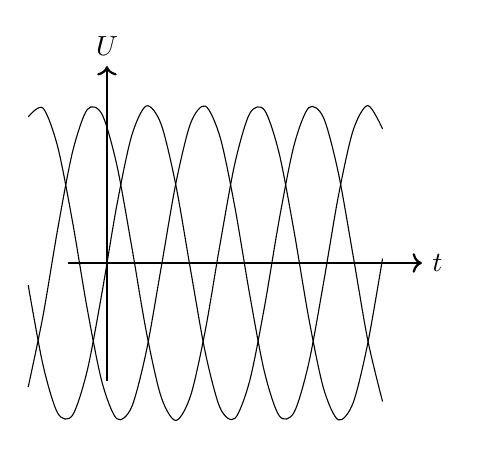
\begin{tikzpicture}
            %\draw[very thin,color=gray] (-0.1,-1.1) grid (3.9,8.1);
            \draw[->,thick] (-0.5,0) -- (4,0) node[right] {$t$};
            \draw[->,thick] (0,-1.5) -- (0,2.5) node[above] {$U$};
            
            \draw[domain=-1:3.5,smooth] plot(\x,{2*sin(3*\x r + 120)});
            \draw[domain=-1:3.5,smooth] plot(\x,{2*sin(3*\x r - 120)});
            \draw[domain=-1:3.5,smooth] plot(\x,{2*sin(3*\x r )});
        
        \end{tikzpicture}
    \caption{波形图}
    \end{minipage}
    \begin{minipage}[t]{0.4\linewidth}
        \centering
        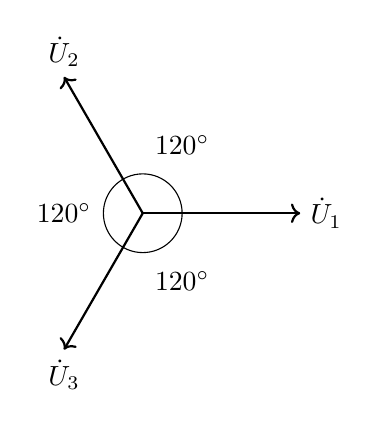
\begin{tikzpicture}
            %\draw[very thin,color=gray] (-0.1,-1.1) grid (3.9,8.1);
            \draw[->,thick] (0,0) -- (2,0) node[right] {$\dot{U}_{1}$};
            \draw[->,thick] (0,0) -- (-1,1.732) node[above] {$\dot{U}_{2}$};
            \draw[->,thick] (0,0) -- (-1,-1.732) node[below] {$\dot{U}_{3}$};
            %\draw (0.5,0) arc (0:120:0.5) node[right] {$120^\circ$};
            %\draw (0.5,0) arc (0:-120:0.5) node[right] {$120^\circ$};
            \draw (0,0) circle (0.5);
            \node at (0.5,0.866) {$120^\circ$};
            \node at (0.5,-0.866) {$120^\circ$};
            \node at (-1,0) {$120^\circ$};
        \end{tikzpicture}
        \caption{向量图}
    \end{minipage}
\end{figure}

\subsubsection{三相电源的星形联结}

如下图所示,三相绕组的三个末端接在一起,与三个首段一起向外引出
四根供电线,或只从三个首段引出三根供电线,称为三相电源的星形联结。
前者称作三相四线制,后者称作三相三线制。

\begin{center}
    \begin{circuitikz}[american voltages]
        \draw
        (0,0) node[anchor=east] {N}
        to [american inductor, *-] (0,2)
        to [short, -o] (5,2) node[anchor=west] {$\text{L}_1$} ;
        \draw
        (0,0)
        to [short, -o] (5,0) node[anchor=west] {$\text{N}$} ;
        \draw
        (0,0)
        to [american inductor, *-] (1.732,-1)
        to [short, -o] (5,-1) node[anchor=west] {$\text{L}_2$} ;
        \draw
        (0,0)
        to [american inductor, *-] (-1.732,-1)
        to [short] (-1.732,-2) 
        to [short, -o] (5,-2) node[anchor=west] {$\text{L}_3$} ;
    \end{circuitikz}
\end{center}

N为中性点,引出的导线称为中性线,又称零线。
由L1、L2、L3引出的导线称为相线或端线,俗称火线。\\
相电压:相线与中位线之间的电压,用$U_{1},U_2,U_3$表示。\\
线电压:两相线之间的电压,用$U_{12},U_{23},U_{31}$表示。

\begin{equation}
    \begin{aligned}
        \dot{U}_{12} &= \dot{U}_{1} - \dot{U}_{2} \\
        \dot{U}_{23} &= \dot{U}_{2} - \dot{U}_{3} \\
        \dot{U}_{31} &= \dot{U}_{3} - \dot{U}_{1}
    \end{aligned}
\end{equation}

\noindent 用$U_P$表示相电压有效值,$U_L$表示线电压有效值,电压对称情况下有:

\begin{equation}
        U_l=\sqrt{3}U_P
\end{equation}

\noindent 相电流:每相绕组的电流,用$I_1,I_2,I_3$表示。

\noindent 线电流:端点输出的电流,用$I_{L1},I_{L2},I_{L3}$表示。

\begin{equation}
    \begin{aligned}
        \dot{I}_{L1} &= \dot{I}_{1} \\
        \dot{I}_{L2} &= \dot{I}_{2} \\
        \dot{I}_{L3} &= \dot{I}_{3}
    \end{aligned}
\end{equation}

\noindent 用$I_P$表示相电流有效值,$I_L$表示线电流有效值,电流对称情况下有:

\begin{equation}
        I_l=I_P
\end{equation}

\subsubsection{三相电源的三角联结}

如下图所示,三相电源中的每相绕组首尾相接,形成一个闭合回路,
然后从连接点引出三根供电线,这种连接方式称为三相电源的三角联结。

\begin{center}
    \begin{circuitikz}[american voltages]
        \draw
        (-1.732,-1)
        to [american inductor, i=$\dot{I}_{1}$, *-] (0,2)
        to [short, -o] (5,2) node[anchor=west] {$\text{L}_1$} ;
        \draw
        (0,2)
        to [american inductor, i=$\dot{I}_{2}$, *-] (1.732,-1)
        to [short, -o] (5,-1) node[anchor=west] {$\text{L}_2$} ;
        \draw
        (1.732,-1)
        to [american inductor, i=$\dot{I}_{3}$, *-] (-1.732,-1)
        to [short] (-1.732,-2) 
        to [short, -o] (5,-2) node[anchor=west] {$\text{L}_3$} ;
    \end{circuitikz}
\end{center}

\noindent 相电压与线电压的关系以及相电流与线电流的关系

\begin{equation}
    \begin{aligned}
        \dot{U}_{1} &= \dot{U}_{12} \\
        \dot{U}_{2} &= \dot{U}_{23} \\
        \dot{U}_{3} &= \dot{U}_{31}
    \end{aligned}
\end{equation}
\begin{equation}
    \begin{aligned}
        \dot{I}_{L1} &= \dot{I}_{1} - \dot{I}_{2} \\
        \dot{I}_{L2} &= \dot{I}_{2} - \dot{I}_{3} \\
        \dot{I}_{L3} &= \dot{I}_{3} - \dot{I}_{1}
    \end{aligned}
\end{equation}



\subsection{三相负载}

\noindent 每相负载首末端之间的电压称为相电压。\\
两相负载首端之间的电压称为线电压。

\noindent 相电压与相电流之间的关系

\begin{equation}
    \begin{aligned}
        \dot{U}_{1} &= \dot{Z}_{1} \dot{I}_{1} \\
        \dot{U}_{2} &= \dot{Z}_{2} \dot{I}_{2} \\
        \dot{U}_{3} &= \dot{Z}_{3} \dot{I}_{3}
    \end{aligned}
\end{equation}

\noindent \textbf{对称三相电路中,中性线的电流为零。\\
中性线的作用:保持负载中性点和电源中性点电位相同。从而在
三相负载不对称时,负载的相电压仍是对称的。}


\subsection{触电防护}

了解安全电压,保护接地、保护接零(IT系统,TN系统,TT系统),漏电开关。

\section{变压器}

\subsection{磁路}

常用物理量:磁通量$\varPhi $,单位韦伯(Wb);
磁通量密度$B$,单位特斯拉(T);
磁场强度$H$,单位安培/米(A/m);
磁导率$\mu = \frac{B}{H}$,单位亨利/米(H/m)。

\

\noindent 磁性能:高导磁性;磁饱和性;磁滞性。

\

\noindent 磁路欧姆定律:
\begin{equation}
    \varPhi = \frac{F}{R_m}
\end{equation}

\noindent 其中$R_m$为磁路的磁阻。
\[
    R_m = R_{mc}+R_{m0}=\frac{l_c}{\mu _c A_c}+\frac{l_c}{\mu _cA_c}
\]
$F$为磁动势,等于线圈匝数$N$乘以电流$i$,即
\[F=NI\]

\subsection{电磁铁}

\subsubsection{直流电磁铁}

\textbf{电路}

\noindent 电流$I$只与线圈电压$U$和线圈电阻$R$有关,即
\[I=\frac{U}{R}\]
功耗仅有线圈电阻$R$的功耗,即
\[P=UI=I^2R=\frac{U^2}{R}\]

\textbf{吸力}

衔铁吸合后$\rightarrow R_m  \downarrow \rightarrow\varPhi  \uparrow \rightarrow$吸引力$\uparrow$

\subsubsection{交流电磁铁}

线圈中通过交变电流,由电磁感应定律知,线圈中会产感应
电动势。有以下关系:
\begin{equation}
    e = 2\pi fN\varPhi _m\sin (\omega t-90^\circ) = E_m sin (\omega t-90^\circ)
\end{equation}
在数值上,有效值$E$为:
\begin{equation}
    E = \frac{E_m}{\sqrt{2}}=\frac{2\pi Nf\varPhi _m}{\sqrt{2}} = 4.44Nf\varPhi _m 
\end{equation}
用相量表示为:
\begin{equation}
    \dot{E} = -j4.44Nf\dot{\varPhi} _m
\end{equation}

电路的功率关系与一般的交流电路相同,即
\begin{equation}
    \begin{aligned}
        S &=UI \\
        Q &=UI\sin \varphi \\
        P &=UI\cos \varphi    
    \end{aligned}
\end{equation}

$P$包含铜损$P_{Cu}$和铁损$P_{Fe}$,铁损又包含磁滞损
耗$P_h$和涡流损耗$P_e$。有以下关系:
\begin{equation}
    \begin{aligned}
        P_{Cu} &= RI^2 \\
        P &= P_{Cu}+P_{Fe} \\
        P_{Fe} &= P_h+P_e
    \end{aligned}
\end{equation}

\begin{equation}
    \begin{aligned}
        \dot{I}_{L1} &= \dot{I}_{1} - \dot{I}_{2} \\
        \dot{I}_{L2} &= \dot{I}_{2} - \dot{I}_{3} \\
        \dot{I}_{L3} &= \dot{I}_{3} - \dot{I}_{1}
    \end{aligned}
\end{equation}

\noindent 吸力

衔铁吸合后,电磁吸力的最大值和平均值基本不变,但励磁电流
变小。一般来说交流电磁铁的启动电流比工作电流大很多。

\subsection{变压器}
\begin{center}
    记$k=\frac{N_1}{N_2}$,则在不考虑损耗的情况下有下列关系
\end{center}

% Please add the following required packages to your document preamble:
% \usepackage{graphicx}
\begin{table}[!htbp]
    \centering
    \resizebox{0.5\textwidth}{!}{%
    \begin{tabular}{cc}
    \hline
    电压变换 & $\frac{U_1}{U_2}=\frac{N_1}{N_2}=k$ \\
    电流变换 & $\frac{I_1}{I_2}=\frac{N_2}{N_1}=\frac{1}{K}$ \\
    阻抗变换 & $\left\lvert Z_e\right\rvert =\frac{U_1}{I_1}=k^2\left\lvert Z_L\right\rvert $ \\
    功率传递 & $S_N=U_{N2}I_{N2}=U_{N1}I_{N1}$ \\ \hline
    \end{tabular}%
    }
\end{table}
\section{电动机}
\subsection{三相异步电机的工作原理}

\begin{enumerate}
    \item 旋转磁场
    \begin{enumerate}
        \item 旋转磁场的产生\\
        旋转磁场是由三相交流电通过三相绕组,或多相电流通过多相绕组产生的。
        \item 旋转磁场的转速\\
        磁场的转速被称为同步速度,记作$n_0$,有下式
        \begin{equation}
            n_0=\frac{60f}{p}
        \end{equation}
        \item 旋转磁场的转向\\
        旋转磁场的转向与电流的相序相同,电流的相序决定了旋转磁场的转向。若
        要调转转向,只需调换任意两相电流即可。
    \end{enumerate}
    \item 电磁转矩
    \begin{enumerate}
        \item 电磁转矩的产生 \\
        电磁转矩是由旋转磁场与转子电流的有功分量之间的相互作用产生的。转子转
        速记为$n$,定义转差率$s$为
        \begin{equation}
            s=\frac{n_0-n}{n_0}
        \end{equation}
        \item 电磁转矩的大小 \\
        电磁转矩的大小与旋转磁场磁通量的最大值以及转子电流的有功分量成正比。即
        \begin{equation}
            T\propto\varPhi_{max}I_{2}
        \end{equation}
        可以导出下式
        \begin{equation}
            T=K_T\frac{sR_2U_1^2}{f_1[R_2^2+(sX_2)^2]}
        \end{equation}
        其中$K_T$常数,$R_2$为转子电阻,$X_2$为转子静止不动的漏电抗,
        $sX_2$为转子转动的漏电抗。
        \item 电磁转矩的方向 \\
        电磁转矩的方向与旋转磁场方向相同。
    \end{enumerate}
    \item 转矩平衡 \\
    记电磁转矩,空载转矩,负载转矩,输出转矩分别为$T,T_0,T_L,T_2$。则有
    \begin{equation}
        T_2=T-T_0
    \end{equation}
    转矩平衡方程
    \begin{equation}
        T_2=T_L,\text{即} T=T_0+T_L
    \end{equation}
    \item 功率传递
    输出功率
    \begin{equation}
        P_2=T_2\omega=\frac{2\pi}{60}T_2n
    \end{equation}
    输入功率
    \begin{equation}
        P=\sqrt{3}U_{1L}I_{1L}\lambda=3U_{1P}I_{1P}\lambda
    \end{equation}
\end{enumerate}

\subsection{三相异步电机的基本结构}

\begin{enumerate}
    \item 定子
    \begin{enumerate}
        \item 定子铁心\\
        定子铁心是由硅钢片叠压而成的,用于减小铁心的磁滞损耗和涡流损耗。
        \item 定子绕组\\
        定子绕组是由若干根绕组线并联而成的,绕组线的截面积越大,电阻越小,电流
        越大,定子铜耗越小。
    \end{enumerate}
    \item 转子
    \begin{enumerate}
        \item 转子铁心\\
        转子铁心是由硅钢片叠压而成的,用于减小铁心的磁滞损耗和涡流损耗。
        \item 转子绕组\\
        转子绕组是由若干根绕组线串联而成的,绕组线的截面积越大,电阻越小,电流
        越大,转子铜耗越小。
    \end{enumerate}
    \item 端盖\\
    端盖是用于固定定子绕组和转子绕组的。
    \item 机座\\
    机座是用于固定定子和转子的。
\end{enumerate}

\subsection{三相异步电机的铭牌数据}

\begin{enumerate}
    \item 型号 (会认磁极数)
    \item 额定功率 $P_N$
    \item 额定电压 $U_N$
    \item 额定电流 $I_N$
    \item 额定转速 $n_N$
    \item 额定频率 $f_N$
    \item 额定功率因数 $\lambda_N$
    \item 绝缘等级
\end{enumerate}

\subsection{三相异步电机的机械特性}

\begin{enumerate}
    \item 固有特性
    \begin{enumerate}
        \item 额定状态 \\
        额定状态是指电机在额定电压,额定频率,额定转速,额定功率下
        的工作状态
        \begin{equation}
            T_N=\frac{P_N}{\omega_N}=\frac{60}{2\pi}\frac{P_N}{n_N}
        \end{equation}
        \item 临界状态
        电动机的电磁转矩等于最大值时的状态。
        
        临界转差率 $s_{M}$
        \begin{equation}
            s_{M}=\frac{R_2}{X_2}
        \end{equation}
        最大转矩
        \begin{equation}
            T_{M}=K_T\frac{U_1^2}{2f_1X_2}
        \end{equation}
        \item 启动状态
        电动机在启动时,还未转动的状态。
        区分过载倍数$K_M$,启动转矩倍数$K_S$,启动电流倍数$K_C$。

        能否启动的判断:起动转矩大于负载转矩;起动电流小于允许最大电流。

    \end{enumerate}
    \item 人为特性 (在书上看)
    \begin{enumerate}
        \item 定子电压降低人为特性
        \item 转子电阻增加人为特性
    \end{enumerate}
\end{enumerate}

\subsection{三相异步电机的启动方法}

\begin{enumerate}
    \item 直接启动
    \item 降压启动
    \begin{enumerate}
        \item 自耦变压器降压启动\\
        $K_A$w为自耦变压器的变压比,启动电流减小$K_A$倍;
        从电源取用的电流和启动转矩减小$K_A^2$倍。
        \item 星形-三角形降压启动\\
        起动电流、电源电流和起动转矩只有直接启动的$1/3$。
    \end{enumerate}
    \item 软启动
\end{enumerate}

\subsection{三相异步电机的调速}

\begin{enumerate}
    \item 变频调速
    \item 变极数调速
    \item 变压调速
    \item 转子电路串联电阻调速
\end{enumerate}
\section{电气自动控制}

\newpage
\end{document}
